% Architecture diagram for the Kafka order pipeline.
% Build:  pdflatex architecture.tex
% To PNG: pdftocairo -png -r 300 -singlefile architecture.pdf architecture
\documentclass[border=14pt]{standalone}

\usepackage[T1]{fontenc}
\usepackage[scaled=0.92]{helvet}
\renewcommand\familydefault{\sfdefault}

\usepackage{tikz}
\usetikzlibrary{arrows.meta,positioning,calc}

% --- palette ---------------------------------------------------------------
\definecolor{inkDark}{HTML}{1F2933}
\definecolor{inkMid}{HTML}{52606D}
\definecolor{lineGrey}{HTML}{9AA5B1}

\definecolor{prodFill}{HTML}{E3F0FC}\definecolor{prodEdge}{HTML}{2A6FB0}
\definecolor{topicFill}{HTML}{ECEFF3}\definecolor{topicEdge}{HTML}{52606D}
\definecolor{consFill}{HTML}{E4F5EC}\definecolor{consEdge}{HTML}{2E7D52}
\definecolor{aggFill}{HTML}{EFE9F8}\definecolor{aggEdge}{HTML}{6B4FA8}
\definecolor{retryFill}{HTML}{FDF1DC}\definecolor{retryEdge}{HTML}{B77A12}
\definecolor{dlqFill}{HTML}{FBE6E6}\definecolor{dlqEdge}{HTML}{B3352F}

\begin{document}
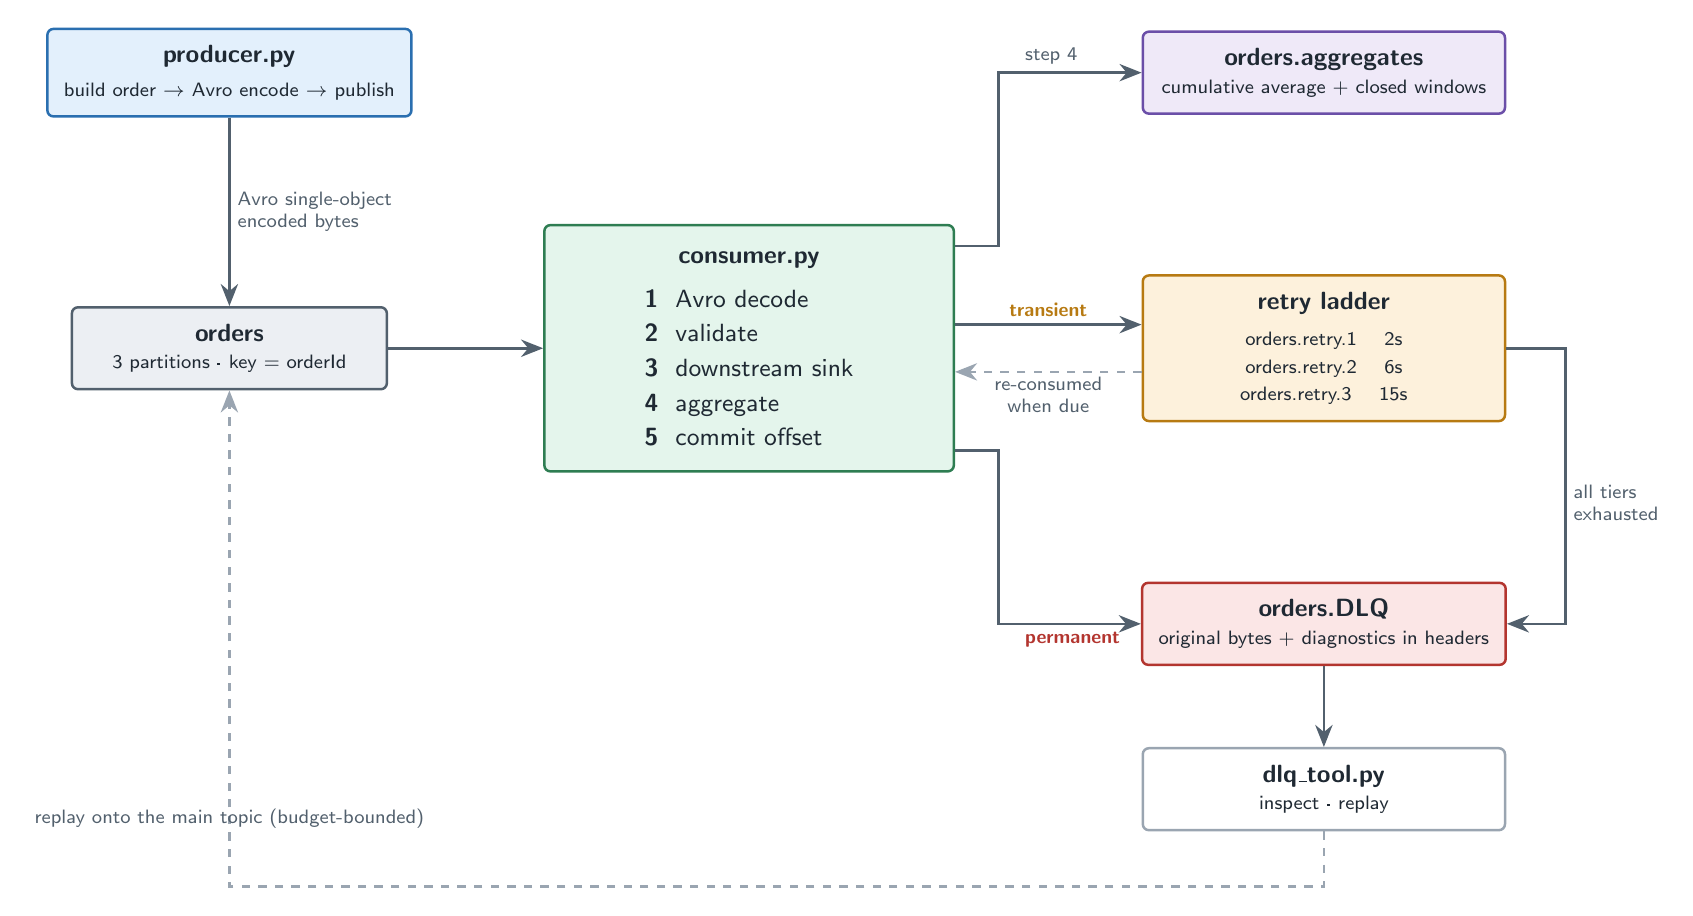
\begin{tikzpicture}[
  font=\small,
  box/.style={
    rectangle, rounded corners=2.2pt, draw, line width=0.9pt,
    align=center, inner sep=6pt, text=inkDark},
  producer/.style={box, fill=prodFill, draw=prodEdge, minimum width=40mm},
  topic/.style={box, fill=topicFill, draw=topicEdge, minimum width=40mm},
  consumer/.style={box, fill=consFill, draw=consEdge, minimum width=52mm},
  agg/.style={box, fill=aggFill, draw=aggEdge, minimum width=46mm},
  retry/.style={box, fill=retryFill, draw=retryEdge, minimum width=46mm},
  dlq/.style={box, fill=dlqFill, draw=dlqEdge, minimum width=46mm},
  tool/.style={box, fill=white, draw=lineGrey, minimum width=46mm},
  flow/.style={-{Stealth[length=2.8mm,width=2.2mm]}, line width=0.95pt, draw=inkMid},
  faint/.style={-{Stealth[length=2.8mm,width=2.2mm]}, line width=0.85pt,
                draw=lineGrey, dashed},
  lbl/.style={font=\scriptsize, text=inkMid, inner sep=2.5pt},
  tag/.style={font=\scriptsize\bfseries, inner sep=2.5pt},
]

% =============================== nodes =====================================
\node[producer]  at (0,3.5)     (prod)   {\textbf{producer.py}\\[1pt]
  {\scriptsize build order $\rightarrow$ Avro encode $\rightarrow$ publish}};

\node[topic]     at (0,0)       (orders) {\textbf{orders}\\[-1pt]
  {\scriptsize 3 partitions \textperiodcentered{} key = orderId}};

\node[consumer]  at (6.6,0)     (cons)   {%
  \begin{tabular}{@{}l@{}}
    \multicolumn{1}{c}{\textbf{consumer.py}}\\[5pt]
    \textbf{1}~~Avro decode\\[1.5pt]
    \textbf{2}~~validate\\[1.5pt]
    \textbf{3}~~downstream sink\\[1.5pt]
    \textbf{4}~~aggregate\\[1.5pt]
    \textbf{5}~~commit offset\\
  \end{tabular}};

\node[agg]       at (13.9,3.5)  (aggr)   {\textbf{orders.aggregates}\\[-1pt]
  {\scriptsize cumulative average + closed windows}};

\node[retry]     at (13.9,0)    (retry)  {\textbf{retry ladder}\\[2pt]
  {\scriptsize orders.retry.1 \quad 2s}\\[-1pt]
  {\scriptsize orders.retry.2 \quad 6s}\\[-1pt]
  {\scriptsize orders.retry.3 \quad 15s}};

\node[dlq]       at (13.9,-3.5) (dlq)    {\textbf{orders.DLQ}\\[-1pt]
  {\scriptsize original bytes + diagnostics in headers}};

\node[tool]      at (13.9,-5.6) (tool)   {\textbf{dlq\_tool.py}\\[-1pt]
  {\scriptsize inspect \textperiodcentered{} replay}};

% =============================== flows =====================================
% producer -> orders
\draw[flow] (prod) -- node[lbl,right,align=left]
  {Avro single-object\\encoded bytes} (orders);

% orders -> consumer
\draw[flow] (orders) -- (cons);

% consumer -> aggregates  (exits high, clears the retry arrows)
\draw[flow] ($(cons.east)+(0,1.3)$) -- ++(0.55,0) |- (aggr.west)
  node[lbl, pos=0.62, above right, xshift=-2mm] {step 4};

% consumer <-> retry ladder: two parallel arrows, opposite directions
\draw[flow] ($(cons.east)+(0,0.30)$) -- ($(retry.west)+(0,0.30)$)
  node[tag, text=retryEdge, midway, above] {transient};
\draw[faint] ($(retry.west)+(0,-0.30)$) -- ($(cons.east)+(0,-0.30)$)
  node[lbl, midway, below, align=center, fill=white, inner sep=1.5pt]
  {re-consumed\\when due};

% consumer -> DLQ  (exits low)
\draw[flow] ($(cons.east)+(0,-1.3)$) -- ++(0.55,0) |- (dlq.west)
  node[tag, text=dlqEdge, pos=0.62, below right, xshift=-2mm] {permanent};

% retry exhausted -> DLQ, routed round the right-hand side
\draw[flow] (retry.east) -- ++(0.75,0) |- (dlq.east)
  node[lbl, pos=0.28, right, align=left] {all tiers\\exhausted};

% DLQ -> tool
\draw[flow] (dlq) -- (tool);

% replay back onto the main topic, routed along the very bottom
\draw[faint] (tool.south) -- ++(0,-0.7) -| (orders.south)
  node[lbl, pos=0.55, above] {replay onto the main topic (budget-bounded)};

\end{tikzpicture}
\end{document}
